Nesta seção são descritos de maneira detalhada a implementação realizada no \textit{benchmark} Bench4Q e a abordagem utilizada no processo de desenvolvimento da extensão. Descrevemos também as implementações das distribuições de carga de trabalho e as disponibilizamos sob uma licença de código aberto, com o intuito de que outros possam reutilizar a plataforma desenvolvida e estender o \textit{benchmark} segundo as suas necessidades para contribuir com outros tipos de modulação de cargas de trabalho num ambiente de experimentos controlado~\footnote{O código fonte está disponível em \href{URL}{http://gitlab.lasdpc.icmc.usp.br/edwin/bench4q}}.

Dentro do processo de experimentos de sistemas de Computação em Nuvem onde é analisado o comportamento da resposta do sistema a uma perturbação no regime transiente, foram identificadas algumas faltas de funcionalidades fundamentais, principalmente na geração da carga de trabalho. Especificamente, o Bench4Q possui algumas limitações na sua versão original, principalmente pela definição do próprio projeto de \textit{software} para avaliação de desempenho no regime estacionário. Esta limitação foi uma barreira que dificultou a experimentação e analise nos trabalhos relacionados com o presente projeto de \citeonline{Edwin2015} e \citeonline{Lourenco2015}.
%As classes disponíveis no \textit{benchmark} original não permitem a modulação de carga de trabalho. Essa limitação implica, por exemplo, na dificuldade de projetar um controlador para o gerenciamento de recursos, pois para esta atividade é necessário uma análise de resultados transientes mediante a modulação da carga de trabalho. A simulação de uma carga de trabalho em que há a alteração introduzida ao longo da simulação é o foco deste trabalho.

No processo de alteração do Bench4Q, foram encontradas classes disponíveis originalmente no \textit{benchmark} que permitem a modulação de carga de trabalho no instante inicial dos experimentos (processo conhecido como processamento em lote). A simulação de uma carga de trabalho em que há a alteração introduzida ao longo do experimento é o foco deste trabalho, as limitações encontradas, por exemplo, dificultam projetar um controlador para o gerenciamento de recursos em tempo real, pois para essa atividade é necessário uma análise de resultados transientes mediante a modulação da carga de trabalho, como foi realizado por \citeonline{nobile2007}. 

O modelo de referência MEDC define um conjunto de requisitos ao qual a presenta proposta de extensão deve-se segui-la e respeitá-la, entre os requisitos, o \textit{Demand}. Segundo \citeonline{Edwin2015}, o requisito \textit{Demand} visa a avaliação de desempenho de sistemas computacionais considerando mudanças na carga de trabalho que chega ao sistema. Para o contexto do Bench4Q, a carga de trabalho são requisições Web que são submetidas à camada de aplicação do \textit{benchmark}. 

O Console do Bench4Q é o módulo que gerencia EBs para gerar uma série sequencial programada de requisições que são submetidas para o SUT. O tópico aqui é controlar a taxa em que os EBs geram as requisições, para que seja possível controlar diretamente e de forma programada a carga de trabalho. Nativamente o Bench4Q, coleta informações sobre a taxa requisições e o comportamento do SUT, e relata esses dados no final da experimento. A Figura \ref{fig:experimental-setup} ilustra de maneira geral o fluxo desse contexto.

\begin{figure}[!htb]
	\centering
	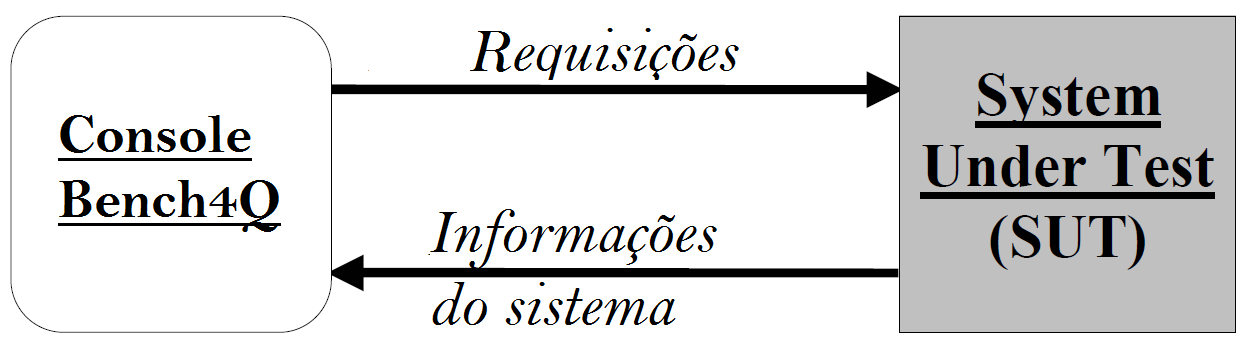
\includegraphics[scale=0.4]{experimental-setup.png}	
	\caption{Configuração experimental Bench4Q.}
	\label{fig:experimental-setup}
	\fadaptada{Vieira2003}
\end{figure}

A extensão implementada na geração de carga do Bench4Q segue a orientação do requisito \textit{Demand} do MEDC, criando novas classes e modificando algumas já existentes da versão original do \textit{benchmark}. Conforme o diagrama de classes na Figura \ref{fig:diagrama-classes}, é possível ter uma ideia de alto nível da extensão realizada no \textit{benchmark}. Vale salientar que o Bench4Q é uma ferramenta completa e extensa, por tais motivos são somente apresentadas algumas das classes mais representativas que passaram por modificações para atender aos requisitos da proposta juntamente às novas classes que foram necessárias para cumprir o objetivo. A Figura \ref{fig:diagrama-classes} mostra o diagrama de classes da extensão do Bench4Q. Como pontos de destaque, as classes sinalizadas na cor azul representam as já existentes, mas que passaram por adaptações e modificações, já as classes na cor verde referem-se as novas classes criadas para possibilitar a modulação da carga do \textit{benchmark}.

O Bench4Q fornece uma estrutura e componentes compartilhados para a comunicação entre os dois módulos da carga de trabalho: \textbf{Console} e \textbf{Agente}. A extensão foi construída inicialmente sob a classe \textsf{MLoadSimulatorPanel}, que orquestra toda a interatividade gráfica do Bench4Q. O novo painel de configuração, que modula a carga, \textsf{MLoadFrequencyPanel} estende a classe original \textsf{Bench4QTreeModel}, adicionando os parâmetros para a modulação como: tipo da carga, o instante em que a carga se inicia, o tempo de atuação da carga e a quantidade de EBs que atuaram nessa carga. O parâmetro \textit{"tipos de carga"}, utiliza da classe enum \textsf{TypeFrequency} que define as constantes dos tipos de modulações programadas para esta extensão.  Todos os parâmetros inseridos na \textsf{MLoadSimulatorPanel} são armazenados na classe \textsf{TestFrequency} que se tornou uma propriedade da classe nativa \textsf{TestPhase}, e que posteriormente são repassadas para a classe \textsf{PropertiesEB} através da \textsf{FrequencySettings}. Já as classes \textsf{Agent}, \textsf{EB}, \textsf{EBClose}, \textsf{EBOpen}, \textsf{Workers}, \textsf{WorkersClosed} e \textsf{WorkersOpen} foram modificadas para receber os novos parâmetros da \textsf{PropertiesEB} gerando a carga programada durante a execução dos experimentos.

\begin{figure}[!htb]
	\centering
	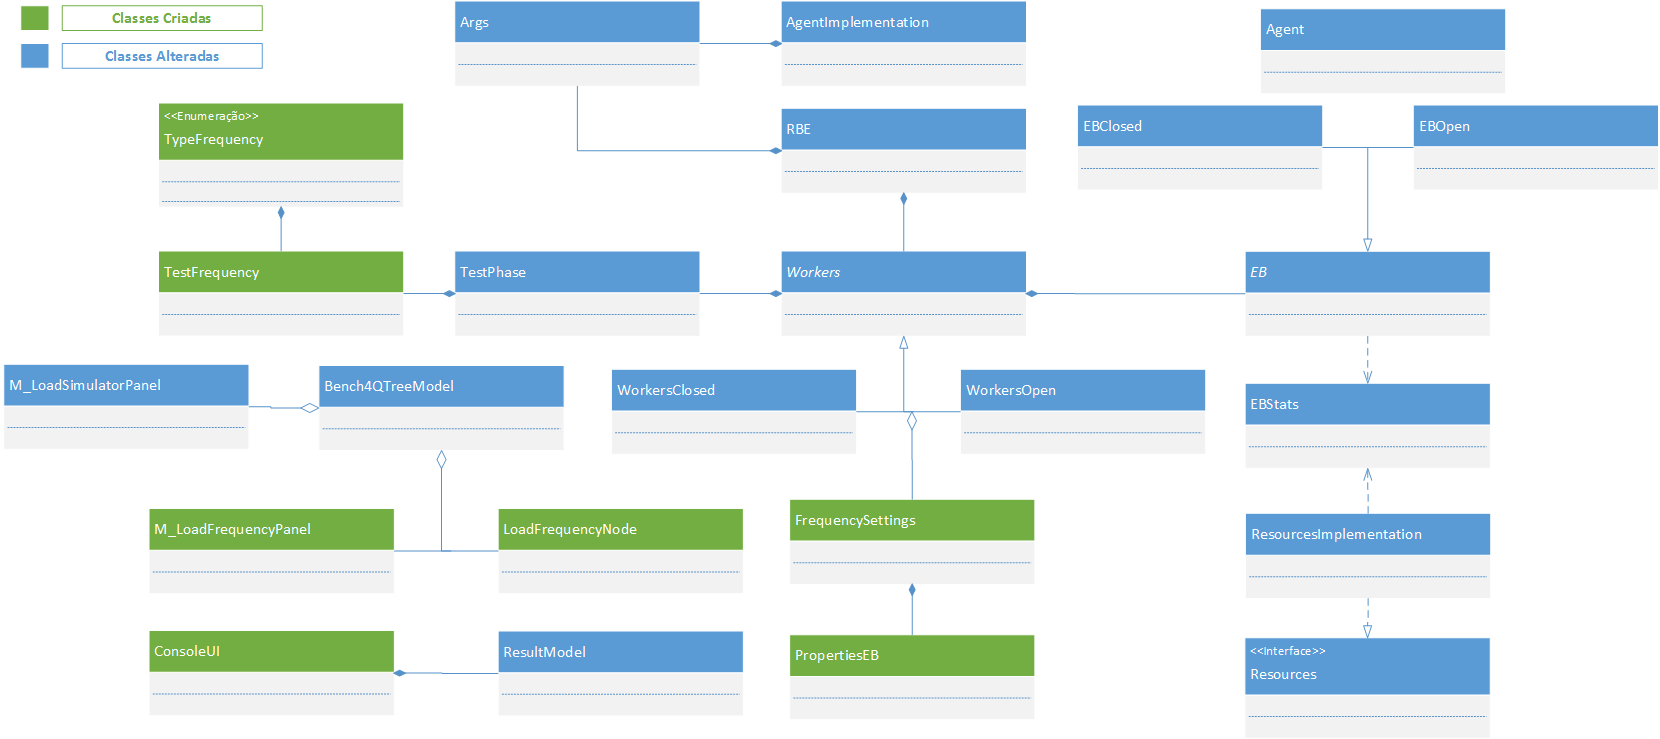
\includegraphics[angle=90, scale=0.6]{diagrama-classes-beanch4Q.png}	
	\caption{Diagrama de classes da extensão do Bench4Q.}
	\label{fig:diagrama-classes}
	\fautor
\end{figure}

O trabalho de desenvolvimento da extensão compreendeu extensivas modificações no código-fonte original do Bench4Q e a criação de novas funcionalidades. Algumas das principais modificações são descritas nas próximas seções.

\section{Configuração da carga de trabalho}
O módulo Agente do Bench4Q está diretamente ligado ao módulo Console do \textit{benchmark} onde são definidas as configurações inicias para os experimentos. Essa caraterística da arquitetura do \textit{benchmark} permite que diversos clientes (Agentes), sejam configurados e gerenciados de maneira organizada, assim como, fornecendo uma potencial escalabilidade para a execução dos experimentos, permitindo variados ambientes com alta ou baixa concorrência ou quantidade de requisições.

O Cliente é um programa Java para gerar as operações que compõem a carga de trabalho. Cada EB é representado por uma \textit{thread} que executa uma série requisições com diferentes \textit{think times} governados por uma função exponencial que finalmente são submetidas ao SUT. Para distribuir e controlar a submissão da carga de trabalho ao longo da simulação, uma estratégia utilizada é a modulação por meio de parâmetros que configuram o comportamento da carga. O cliente tem uma série de propriedades que definem o seu funcionamento e o comportamento resultante da carga de trabalho, apresentados no Capítulo \ref{chapter:metodologia}. 

O pseudo-código \ref{code:createProperties} refere-se a classe \textsf{FrequencySettings} criada para a extensão, que contém o algoritmo responsável por calcular os tempos de inicialização, pause e termino de cada um dos clientes. Este código é o ponto central que resulta no comportamento final da modulação da carga de trabalho. Entre as tarefas encontra-se definir os períodos (\textit{think time}) de execução e interrupção para cada EBs, como um planejamento de tarefas. Para calcular os períodos de execução e interrupção são utilizados outros parâmetros nativo ao Bench4Q como o Tempo de Experimento. O código fonte apresentado na integra pode ser conferido no Apêndice \ref{cap:ap-codigo} código \ref{code:createProperties-all}.

No princípio um conjunto de variáveis ( \textsf{timeStart}, \textsf{timeEnd}, \textsf{timePause} e \textsf{timeExperiment}) são inicializadas, em geral com valores informados previamente e mesurados em milesegundos. A condição IF verifica o tipo de modulação a ser gerada. Em seguida, outra condicional IF verifica, através do index, se o EBs é configurável para a modulação e calculando os tempos de inicializações e interrupções de cada EBs.

\begin{codigo}[caption={Algoritmo calcula os tempos de inicialização e termino para cada um dos Clientes}, label={code:createProperties}, breaklines=true]
	ParametrosExperimento createProperties(Time tempoExperimento) {
		
		ParametrosExperimento parametros = new ParametrosExperimento();
		
		parametros.TempoIncial = calculaTempoInicial();
		parametros.TempoFinal = calculaTempoFinal();
		parametros.TempoPausa = calculaTempoPausa();
		
		retorna parametros;
	}
}
\end{codigo}

Novos tipos de modulações podem ser adicionadas a esta versão do Bench4Q. Isto é especialmente útil para \textit{benchmarks} que têm requisitos muito especiais para a sua validação e/ou análise de desempenho. Por esse motivo foi criada a classe \textsf{FrequencySettings} para que outros tipos de modulações sejam implementadas com os seus cálculos necessários para a sua execução tornando simples a criação de novos tipos de carga de trabalho para outros desenvolvedores. As novas modulações a serem implementadas deve ser incluídas neste método, juntamente com o nome do novo tipo de carga na classe Enum \textit{TypeFrequency}.

\section{Geração da carga de trabalho}
A princípio foi identificado o modulo de geração de carga do Bench4Q e este passou por alterações para gerar a carga de trabalho esperada. Logo, esta classe é nativa do \textit{benchmark}. O Bench4Q tem dois tipos de sessões, \textit{Open} e \textit{Close}, e estas tem grande influência na geração da carga de trabalho. Consequentemente existem duas classes que tratam cada umas das sessões (\textit{WorkersOpen} e \textit{WorkersClose}) com o mesmo métodos, mas com implementações diferentes.
O pseudocódigo \ref{code:modelworkload}, apresentado na a seguir, ilustra o \textit{core} da geração da carga referente a construção da modulação da carga já com as modificações da extensão, este método é o encarregado do gerenciamento da geração dos EBs. Através dos parâmetros e dados calculados anteriormente é possível controlar as requisições afim de gerar as modulações desejas. 

Para maiores detalhes o código-fonte é apresentado na integra no Apêndice \ref{cap:ap-codigo} código \ref{code:modelworkload-all}. O código é extenso, aqui iremos descrever somente os trecho de interesse a modulação da carga de trabalho. O loop nativo \textit{while} repete em quanto o valor \textsf{parametros.ExperimentoEmExecucao} for verdadeiro (\textsf{parametros.ExperimentoEmExecucao}, é o número de transações a serem efetuadas). A primeira condicional IF verifica se o tempo corrente é maior que o tempo de experimento, compreendendo assim a finalização do experimento a interrupção de novas requisições, assim a variável nativa é atribuída com o valor false encerrando as execução (código-fonte \ref{code:modelworkload}: linha 34). Já na segunda condicional IF, é verificado se o tempo corrente é maior que o tempo final de execução do EB somente para os EBs que são moduláveis. Neste caso é verificado, na sub-condicional IF, se existem pausa programadas e calculados novos tempos de execução e interrupção do EB, caso contrário é encerrada a execução do EB com a atribuição false para a variável (código-fonte \ref{code:modelworkload}: linha 14). A terceira condicional IF (código-fonte \ref{code:modelworkload}: linha 25), trata se o tempo corrente é maior ou igual ao tempo de início de execução do EB; para este caso será gerada uma requisição, caso a sub-condicional IF (código-fonte \ref{code:modelworkload}: linha 34) não seja verdadeira, pois esta encerra a execução do EB.


\begin{codigo}[caption={Algoritmo de geração de carga modificado para modulação}, label={code:modelworkload}, breaklines=true]
	ParametrosExperimento parametros;
	ebCorrente.EmExecucao = true;
	while (parametros.ExperimentoEmExecucao) {	
		tempoCorrente = System.pegaTempoCorrente();
		
		if (tempoCorrente > parametros.TempoExperimento){
			ebCorrente.EmExecucao = false;
		}
		
		if (tempoCorrente > ebCorrente.TempoDuracao && ebCorrente.EbMarcado) {
			if(parametros.TempoPausa > 0){			
				long novoInicio = ebCorrente.TempoFinal + parametros.TempoPausa ;
				long periodo = ebCorrente.TempoFinal - ebCorrente.TempoInicial;
				
				ebCorrente.TempoInicial = novoInicio;
				ebCorrente.TempoFinal = periodo + novoInicio;
			} else if (tempoCorrente > ebCorrente.TempoInicial) {
			ebCorrente.EmExecucao = false;
		}
	}
	
	if (tempoCorrente >= ebCorrente.TempoInicio) {
		if (!ebCorrente.EmExecucao) {
			return;
		}
		if (ebCorrente.TemProximaPagina) {
			// fluxo de acesso a pagina do SUT (recurso nativo do Bench4Q)
		} else {
		ebCorrente.EmExecucao = false;
	}	
	if (!ebCorrente.EmExecucao = false;) {
		return;
	} else {
	ebCorrente.Dorme(500);				
}

}
\end{codigo}

Modelagem de carga de trabalho é uma tentativa de criar um modelo simples, que pode então ser utilizada para gerar cargas sintéticas. O objetivo é de ser capaz de criar cargas de trabalho que podem ser utilizados em estudos de avaliação de desempenho com semelhanças as cargas de sistemas reais. 

\section{\textit{Interface} gráfica}

No Console são configurados os parâmetros iniciais para a execução do experimento, foi incluída uma nova opção \textit{LoadFrequency} no menu do Bench4Q, que referente aos parâmetros da extensão da geração da carga. Por esta opção, \textit{LoadFrequency}, deve-se preencher os campos (\textit{Start Time}, \textit{Duration Step}, \textit{Pause} e \textit{Quantity}) que irão gerar a carga conforme a programação. O pseudo-código \ref{code:panel} apresenta a criação da interface gráfica, o método \textit{private} presente na classe \textit{MLoadFrequencyPanel} que cria a \textit{interface} gráfica gerada com a biblioteca \textit{Swing} do Java, toda a parte gráfica do Bench4Q utiliza da mesma biblioteca. Todos os resultados de desempenho de cada agente de carga são agregados no console de carga para análise e demonstração, conforme a versão original. O código fonte pode ser apreciado na integra no Apêndice \ref{cap:ap-codigo} código \ref{code:panel-all}.

\begin{codigo}[caption={Código para gerar a os parâmetros para a modulação}, label={code:panel}, breaklines=true]
	private void createPanelFunction(Menu menu) {
		
		Panel panelLoadFrequency = menu.addItem(novo Panel());
		panelLoadFrequency.setNome("LoadFrequency");
		
		panelLoadFrequency.addCampo("Start Time");
		panelLoadFrequency.addCampo("Duration Step");
		panelLoadFrequency.addCampo("Pause");
		panelLoadFrequency.addCampo("Quantity");	
		
		menu.atualizar();
		menu.reconstruir();
		
	}
\end{codigo}

Este conjunto de classes as quais lidam, manipulam, gerenciam e modulam a carga de trabalho gerada pelo Bench4Q são utilizadas pelo Console para configurar, monitorar e analisar todo o experimento. Todo o desenvolvimento, referente à modificação e implementação de novas classes, mantiveram e respeitaram o padrão de desenvolvimento do \textit{benchmark}. A Figura \ref{fig:interface-criada-beanch4q} ilustra a interface gráfica por onde é possível modular a carga de trabalho do Bench4Q. 

\begin{figure}[!htb]
	\centering
	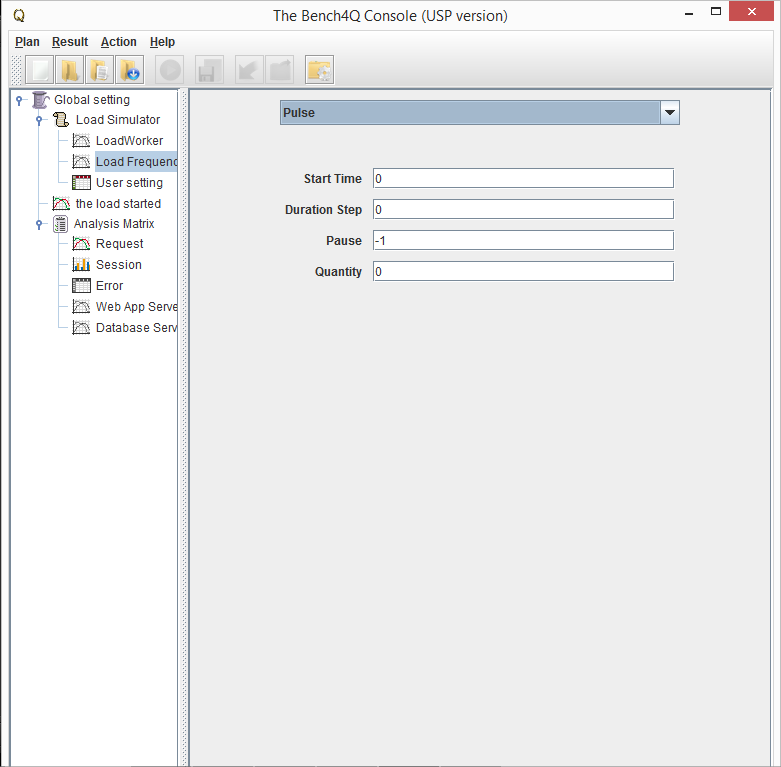
\includegraphics[scale=0.6]{console-bench4Q-usp.png}
	\caption{Console de programação da carga de trabalho.}
	\label{fig:interface-criada-beanch4q}
	\fautor
\end{figure}


\section{Teste de modulação}

A carga de trabalho é imposta ao sistema por meio de requisições HTTP enviadas pelos EBs ao SUT que são processadas nos servidores de aplicação das máquinas virtuais instanciadas no \textit{host}. Essas requisições exigem que as máquinas virtuais se ocupem pelo tempo necessário para processá-las, alterando o desempenho experimentado pelo sistema.
Segundo \citeonline{Nobile2013}, existem dois fatores associados a uma requisição e que afetam diretamente o desempenho do sistema:
%\begin{citacao}
o tempo de processamento e a quantidade de carga imposta pelas requisições, são dados pelo tempo de processamento e pela taxa de chegada de novas requisições, respectivamente. Com o tempo, a quantidade e o tamanho das requisições podem se alterar, dependendo do perfil de utilização dos usuários que utilizam o serviço naquele momento. Havendo um aumento em algum desses fatores é possível que o desempenho do sistema sofra degradação, podendo em casos extremos, entrar em colapso.
%\end{citacao}

É possível informar previamente a execução dos parâmetros da modulação. Por exemplo, ao escolher a opção degrau, é necessário informar quantos EBs geram o degrau, em que instante de tempo, e qual o tempo de duração e por fim qual a sua polaridade (com base em um pulso elétrico a positiva sairia de zero e chega a um, a negativa, sairia de um e chegaria a zero), é possível obter resultados conforme a Figura \ref{fig:grafico-carga-modulada-teste}.

\begin{figure}[!htb]
	\centering
	\begin{subfigure}{\linewidth}
		\centering
		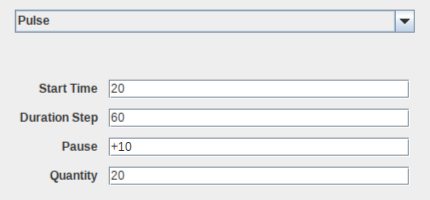
\includegraphics[scale=0.7]{condiguracao-carga-modulada1.png}
		\caption{Teste de configuração da carga a ser modulada}
		\label{fig:configuracao-carga-modulada-teste}
	\end{subfigure}
	
	\begin{subfigure}{\linewidth}
		\centering
		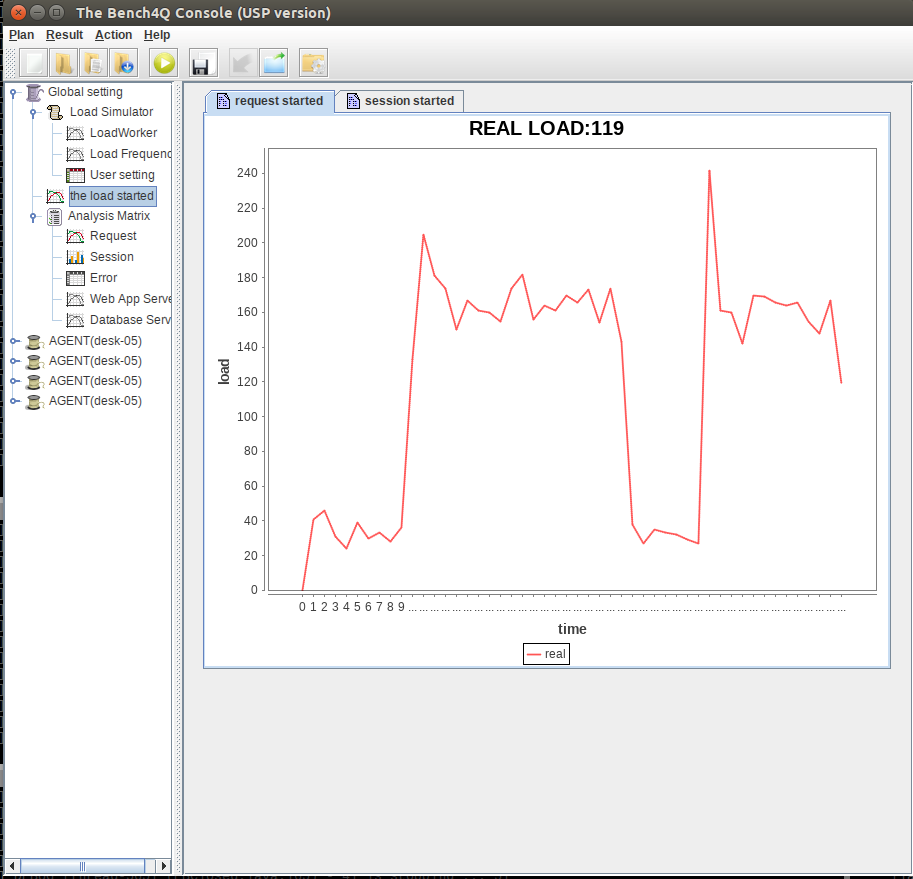
\includegraphics[scale=0.6]{grafico-carga-modulada-teste.png}
		\caption{Carga gerada com base na configuração teste}
		\label{fig:grafico-carga-modulada-teste}
	\end{subfigure}  
	\caption{Teste de modulação da carga}  
	\label{fig:carga-modulada-teste}
	\fautor
\end{figure}  

A Figura \ref{fig:carga-modulada-teste} ilustra uma carga teste modulada já pela extensão. A Figura \ref{fig:configuracao-carga-modulada-teste} apresenta os parâmetros utilizado para realizar o teste. A carga modulada atuará a partir do décimo segundo de experimentação e com uma duração de 20 segundos; com 30 segundos de experimentação ocorrerá uma pausa de 7 segundos e um novo degrau será gerado em seguida, o qual se manterá até o final do experimento. Para este exemplo foram fixados 40 EBs por Agente para modular o comportamento da carga. Este comportamento pode ser apreciado no item \ref{fig:grafico-carga-modulada-teste} da mesma Figura \ref{fig:carga-modulada-teste}. Vale salientar que o gráfico gerado e apresentado na figura \ref{fig:carga-modulada-teste} de item \ref{fig:grafico-carga-modulada-teste}, é uma característica nativa ao \textit{benchmark}.

Foi elaborada uma documentação seguindo os padrões da última versão original do \textit{benchmark} e esta pode ser conferida no apêndice \ref{chapter:documentacao} que traz informações do programa e qual seu objetivo, entradas suportadas e saídas esperadas, exemplo de como executar o programa e tabela descrevendo as principais características.
